In this section, we want to extend our stability analysis to the one-dimensional advection-diffusion equation
\begin{equation}\label{eq: A-D_equation}
u_t(x,t) + au_x(x,t) = du_{xx}(x,t), \quad a\ge0, \ d \ge 0, \qquad x \in \Omega \subset \mathbb R,
\end{equation}
where $a$ is the coefficient of the advection term and $d$ the coefficient of the diffusion term, using the von  \PO{Neumann stability analysis}. %principles.
\PO{After the space discretization, we discretize the advection part with an explicit time-integration scheme and the diffusion with an implicit one}.
The linear stability of the DeC method in PDE contexts was studied for explicit methods for advection equations with FEM spatial discretizations and various stabilization techniques in \cite{michel2021spectral,michel2023spectral}, while in the IMEX context for FEM methods applied to kinetic models in \cite{torlo2020hyperbolic}.
For the ADER method, a von Neumann stability analysis was applied to the original formulation \cite{titarev2007analysis,dematte2020ader}, but not on the modern version that we are studying. \PO{We close this gap with our investigation in the following.}
\subsection{Finite Difference discretization}
\label{sec: spatial_discretization}
We apply spatial discretizations to the spatial derivative operators, namely $\partial_x$ and $\partial_{xx}$. 
We consider a uniformed grid $\Omega_{\Delta x}=\left\{x_j \ : \ x_j = x_0 + j\Delta x, \ j \in \{0,\hdots , J\}\right\}$ with periodic boundary conditions and we denote the approximation of $u(x_j)=u(x_j,t)$ by $w_j$.

To discretize the advection term in \eqref{eq: A-D_equation}, i.e. the first spatial derivative $\partial_xu(x)$, we make usage of the stable finite difference stencils introduced in \cite{Iserles1982}. Assume we discretize $\partial_xu$ at $x_j$ by an $[r,s]$-discretization
\begin{equation}\label{eq: r-s_scheme}
\partial^{[r,s]}_{\Delta x}(u(x_j)) = \frac{1}{\Delta x} \sum\limits_{k=-r}^s \alpha_k w_{j+k},
\end{equation}
with $r,\ s$ such that $\alpha_{j-r}, \alpha_{j+s} \neq 0$.
The maximum order we can achieve with an $[r,s]$- discretization is $q=r+s$ and this discretization actually reaches order $q$ and is unique by setting the coefficients in \eqref{eq: r-s_scheme} as
	\begin{align}\label{eq:def_advection_optimal_stencil}
	\alpha_0&=
	\begin{cases}
	\sum\limits_{k=r+1}^s\frac{1}{k}, & s\ge r+1, \\
	0, & s=r, \\
	\sum\limits_{k=s+1}^r\frac{1}{k}, & r\ge s+1, 
	\end{cases} \qquad
	\alpha_k = \frac{(-1)^{k+1}}{k}\cdot \frac{r!s!}{(r+k)!(s-k)!}, \quad -r\le k \le s, \ k\neq0.
	\end{align}
 It is also proven in \cite{Iserles1982} that these so-called $\textit{optimal-order}$ schemes of order $q$ are stable if and only if $s\le r \le s+2$ for $a>0$.\\
We  involve these stable $\textit{optimal-order}$ schemes into our analysis. 
We introduce upwinding in the choice of the stencils, in particular, we will consider $[r, r +1]$ stencils for odd optimal-order scheme and $[r, r+2]$ stencils for an even optimal-order scheme for the advection part.

For the diffusion term, we will just use a central finite difference discretization of the second spatial derivative $\partial_{xx} u(x)$ given in Table~\ref{tab: CFD-schemes_first_deriv}.
\begin{table}
	\centering
	\caption{Central finite difference discretizations of $\partial_{xx}$ applied onto $w$ centered in $j$  \cite{fornberg_finite_difference}}
	\label{tab: CFD-schemes_first_deriv}
	\small
	\begin{tabular}[h]{|c|c|}
		\hline
		order & finite difference for $\partial_{\Delta x}^2(u(x_j))$\\
		\hline
		2 & $\frac{1}{\Delta x^2}\left(w_{j-1}-2w_j+w_{j+1}\right)$\\
		\hline
		4 & $\frac{1}{\Delta x^2}\left( -\frac{1}{12}w_{j-2} +\frac{4}{3}w_{j-1} -\frac{5}{2}w_j   +\frac{4}{3}w_{j+1}  -\frac{1}{12}w_{j+2}\right)$\\
		\hline
		6 & $\frac{1}{\Delta x^2}\left(\frac{1}{90}w_{j-3} - \frac{3}{20}w_{j-2} + \frac{3}{2}w_{j} - \frac{49}{18}w_{j} + \frac{3}{2}w_{j} - \frac{3}{20}w_{j+2} + \frac{1}{90}w_{j+3}\right)$\\
		\hline
		8 & $\frac{1}{\Delta x^2}\left(
		-\frac{1}{56}w_{j-4} + \frac{1}{420}w_{j-3} - \frac{1}{5}w_{j-2} + \frac{8}{5}w_{j-1} - \frac{205}{72}w_{j} + \frac{8}{5}w_{j+1} - \frac{1}{5}w_{j+2} + \frac{1}{420}w_{j+3} - \frac{1}{56}w_{j+4}
		\right)$\\
		\hline
	\end{tabular}
\end{table}

\subsection{von Neumann analysis}
\label{sec: stability_theory_PDE}
To analyze the stability of the described methods, we make use of the von Neumann stability analysis for linear partial differential equations \cite{leveque2007finite}.
%\subsubsection{von Neumann Stability}
Briefly summarized, we investigate the behavior inside the numerical scheme of the Fourier modes
\begin{equation}\label{eq: fourier_modes}
w^n_j = v^ne^{ikx_j},
\end{equation}
where $w^n_j$ is the discretization of $u(x_j, t_n)$ and $k$ is the wavenumber and we focus on the representation coefficient $v^n$. 
Indeed, $e^{ikx}$ are eigenfunctions of the differential operator $\partial_x$ and therefore for any linear differential operator. 
If we use \eqref{eq: fourier_modes} in our discretized system, we obtain a system of the form
\begin{equation}
\label{eq: ampfactor}
v^{n+1}=G(k, \Delta x, \Delta t, a, d)v^n.
\end{equation}
with the amplification factor $G\in \mathbb{C}$ independent on the mesh point $x_j$.
%Now, to check the stability of the scheme, we need that $\lvert{v^{n+1}}\rvert= \lvert{G(k, \Delta x, \Delta t, a, d)v^n}\rvert \leq \lvert v^n\rvert$. 
\PO{Stability means in our context that $\lvert{v^{n+1}}\rvert= \lvert{G(k, \Delta x, \Delta t, a, d)v^n}\rvert \leq \lvert v^n\rvert$ holds.}
In practice, we check that $\lvert G (k, \Delta x, \Delta t, a, d) \rvert \le 1$. \PO{This implies stability for the related method and due to the  Lax-Richtmeyer theorem \cite{leveque2007finite} convergence can be ensured.}
Note that for consistency, we included the parameters $a$ and $d$ into the dependency of $G$ to cover all advection-diffusion equations. \\
% This theory concludes in the following condition: 
%\begin{prop}\textbf{Richtmyer condition}\\
%	A finite difference scheme equipped with a time-stepping method is stable in the stability area $\Lambda$ if and only if there exists a constant $K$, such that
%	\begin{equation*}
%	\lvert G (k, \Delta x, \Delta t, a, d) \rvert \le 1+ K \Delta t
%	\end{equation*}
%	with $(k, \Delta x, \Delta t, a, d)\in \Lambda$. 
%\end{prop}
%Remark that for consistency, we included the parameters $a$ and $d$ into the dependency of $G$ to cover all advection-diffusion equations. When we evaluate the amplification factors numerically later on, we will probe the slightly more strict von Neumann condition $\lvert G (k, \Delta x, \Delta t, a, d) \rvert \le 1$ for stability. \\
%This whole analysis gains its relevance based on the following statement.
%\begin{theorem}\textbf{Lax-Richtmyer}\\
%	A consistent finite difference scheme for a partial differental equation with a well-posed inital value problem is convergent if and only if its stable.
%\end{theorem}
%%%%%%%%%%%%%%%%%
%Displaying Stability
%%%%%%%%%%%%%%%%%
Typically, in order to estimate the stability of the advection-diffusion equation, an analytical study of $G$ in all the parameters should be performed. 
This is not feasible when considering high order schemes as ADER and DeC.
Hence, we will evaluate the amplification factor numerically, similarly to what we did with the stability functions in the ODE case.

Before running all the simulations, we need to understand what are the free variables of the function $G$. First of all, the wavenumbers  should be bounded $k \in \lbrace -n_0-1 , \dots, n_0+1 \rbrace \subset \mathbb Z$ and the maximum wavenumber $n_0+1$ is strongly related with the discretization scale $\Delta x$. Indeed, by  Nyquist–Shannon sampling theorem, only functions with frequency less than $\frac{|x_J-x_0|}{2\Delta x}$ can be represented on our discretization. Hence, we will choose $n_0=10^3$ to take in consideration fine grids.

Then, we have further variables $a,d,\Delta x,\Delta t $ that are often coupled together: in the advection term ($a\Delta t/\Delta x$) and in the diffusion term ($d\Delta t/\Delta x^2$). We keep this in mind when studying the behavior of $G$, as we can recast few methods to the same coefficients.

\subsubsection{Displaying stability}
It is stated and numerically shown in \cite{TanChenShu_ImEx_Stability, WangShuZhang_LDG1_2015,WangShuZhang_LDG_2016} that several schemes as the local discontinuous Galerkin scheme \cite{WangShuZhang_LDG1_2015,WangShuZhang_LDG_2016} and other finite difference schemes combined with an IMEX RK method are stable if the time step is upper bounded by some $\tau_0$. This $\tau_0$ is proportional to $\frac{d}{a^2}$, i.e., if $\Delta t\le\tau_0= E_0\cdot \frac{d}{a^2}$ for some $E_0>0$.
%%%%%%%%%%%%%%%%%
%C, D, E Approach
%%%%%%%%%%%%%%%%%
Considering the before mentioned parameters $\Delta x, \Delta t, a,d$, we introduce two new coefficients
\begin{equation}
C=\frac{a\Delta t}{\Delta x}, \quad D=\frac{d\Delta t}{{(\Delta x)}^2}.
\end{equation}

Moreover, using the coefficients $C$ and $D$ reveals an equivalent condition to \cite{TanChenShu_ImEx_Stability}, if we assume that the quotient
\begin{equation*}
E:=\frac{C^2}{D}= \frac{ \Delta t ^2 a^2 }{\Delta x^2} \frac{\Delta x^2}{d \Delta t} = \frac{a^2}{d}\Delta t
\end{equation*}
is bounded by some constant $E_0$, indeed,
\begin{equation*}
E= \frac{a^2}{d}\Delta t\le E_0 \quad \Longleftrightarrow \quad \Delta t \le E_0 \cdot \frac{d}{a^2}=\tau_0.
\end{equation*}
Therefore, for a given method solving the advection-diffusion equation, we can rewrite the amplification factor  with \eqref{eq: ampfactor} as
\begin{equation}
	g(k,C,E)=G(k,\Delta x, \Delta t, a,d).
\end{equation}

\begin{definition}[Scheme notation]	\label{defi: notation_pde_method}
	To shorten the notation, we denote the considered method for the advection-diffusion equation by $[\TMM,\NODES,N, A_n,D_m],$ where
	\begin{itemize}
		\item $\TMM$ stands for the respective IMEX time-marching method, i.e. $\DeC$, $\ADER$, $\sDeC$,
		\item $\NODES$ stands for the used quadrature nodes for the \TMM, i.e. {\eq} or $\GLB$,
		\item $N$ stands for the order of the considered time-marching method $\TMM$,
		\item $A_n$ denotes the optimal first derivative stencil of order $n$ defined in \eqref{eq:def_advection_optimal_stencil} used for the advection term,
		\item $D_m$ denotes the central second derivative stencil of order $m$ in Table~\ref{tab: CFD-schemes_first_deriv} used for the diffusion term.
	\end{itemize}
\end{definition}


\begin{remark}
	With the previous plots, we recognize two sufficient conditions to obtain stability:
	\begin{itemize}
		\item the well known CFL-condition, i.e., if $C$ is lower than some constant $C_0$ only dependent on the method, then the method is stable.
		\item the new numerically obtained condition, designated as the $E_0$-condition: If $E$ is lower than some constant $E_0$ dependent on the method, then the method is stable.
	\end{itemize}
	
	These two parameters $C$ and $E$ include all the remaining ones and show therefore a full picture.
\end{remark}

As we can see in Figure~\ref{fig: exa_ImExDeC3_diff2_adv1}, the unstable area of this specific method seems to be bounded by the linear constraints $C\geq C_0$ and $E\geq E_0$. We will observe numerically that these unstable regions are indeed similarly bounded in most of our methods.
\begin{definition}[Stability parameters $C_0$ and $E_0$]
	Given the amplification factor $g(k,C,E)$ of a discretization of the advection-diffusion equation, we define the two stability parameters $C_0$ and $E_0$ by
	\begin{itemize}
		\item $C_0:=\max_{C\in \mathcal{S}} C$ with $\mathcal{S}=\lbrace C: \lvert g(k,C,E)\rvert \leq 1, \, \forall E>0, \,\forall k \in [-n_0-1,n_0+1] \rbrace$,
		\item $E_0:=\max_{E\in \mathcal{R}}E$ with $\mathcal{R}= \lbrace E: \lvert g(k,C,E)\rvert \leq 1,\, \forall C>0,\,\forall k \in [-n_0-1,n_0+1]\rbrace .$
	\end{itemize}
\end{definition}
Therefore, the strategy we want to follow is to look at the areas of stability by evaluating the amplification factor $\max_k |g(k,C,E)|$ like in Figure~\ref{fig: exa_ImExDeC3_diff2_adv1} and numerically calculating the parameters $C_0$ and $E_0$ for our methods, when possible.

Note, that the condition $E<E_0$ does not depend on $\Delta x$ and avoids CFL restrictions. We should always keep in mind that our numerical evaluations can just cover finite ranges of $C$ and $E$. 
Hence, we checked that the displayed limits for $E$ and $C$ are actually bounds also for larger domains of $C$ and $E$.
Moreover, we also observed that the considered results do not vary much for large values of $n_0$, hence, we set $n_0=10^3$. Due time-efficiency, we will use this value for every evaluation in the von Neumann stability analysis context for the rest of this work. Further, all plots in this section will be evaluated and displayed at $400\times 400$ grid points.
\subsubsection{Numerical analysis}
%To distinguish the different orders, we use different colors to the  bounds according to the legend figure~\ref{fig: legend_a-d}. 
In the following plots, we remark that the colors are assigned to different orders, indeed, we will vary alternatively the order of the advection method, of the time-marching, of the diffusion method or of all of them. We will specify for each plot what is the object of the study.
%\begin{figure}
%	\centering
%	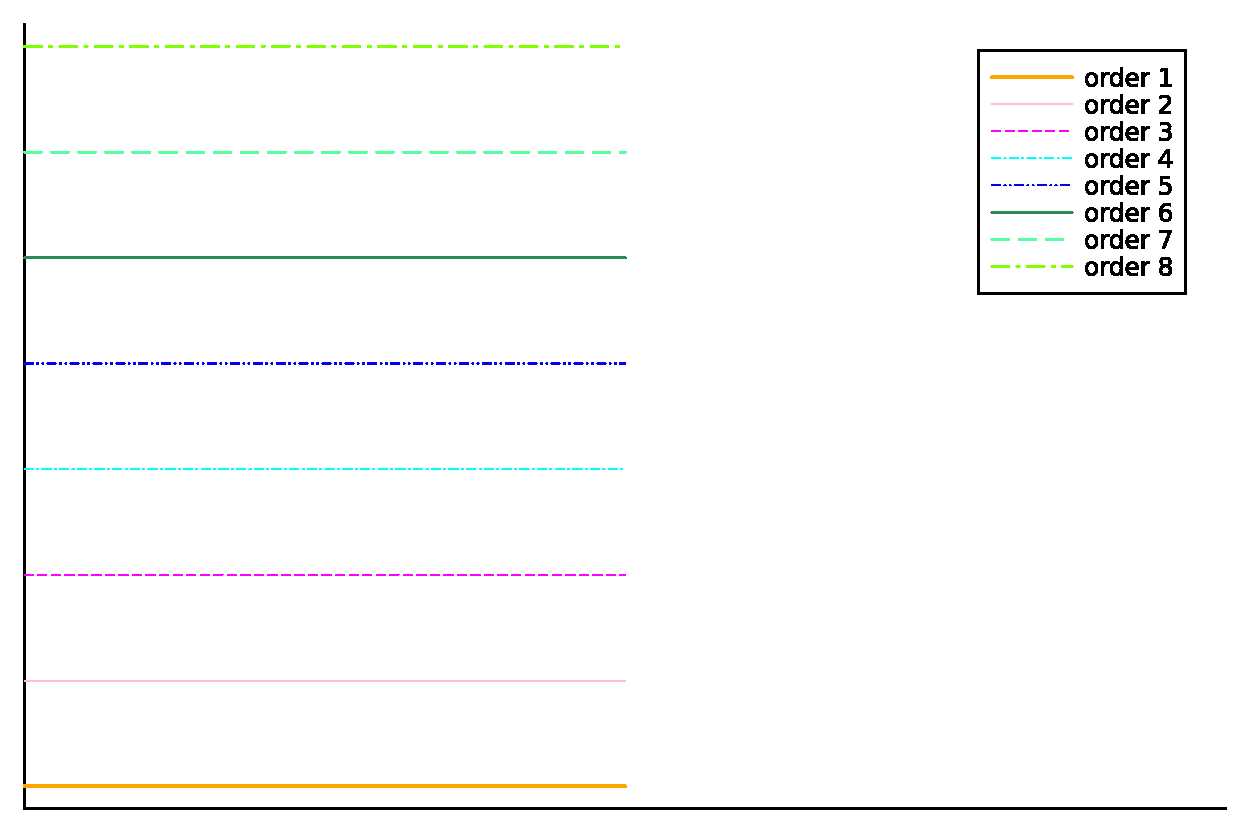
\includegraphics[width=0.17\textwidth, trim={461 256 30 23}, clip]{pdf/odepics/colors_a-d_new_1-8.pdf}
%	\caption{Legend for the different orders.}
%	\label{fig: legend_a-d}
%\end{figure}

We start by varying only the time scheme order. 
In Figure~\ref{fig: grp_adv1_diff2}, the stability areas of several methods are shown, i.e., $[\TMM,\NODES,k, A_1,D_2]$ varying the time scheme and the nodes. 
As in Figure~\ref{fig: exa_ImExDeC3_diff2_adv1}, the plotted lines separates the stable region in the lower left part from the unstable region in the upper right side of the $C$-$E$ plane. 
We see a similar behavior for mostly all methods. 
Increasing the order of the time marching method results in a larger stability region and in larger values for $E_0$ and $C_0$. 

\begin{figure}
	\centering
	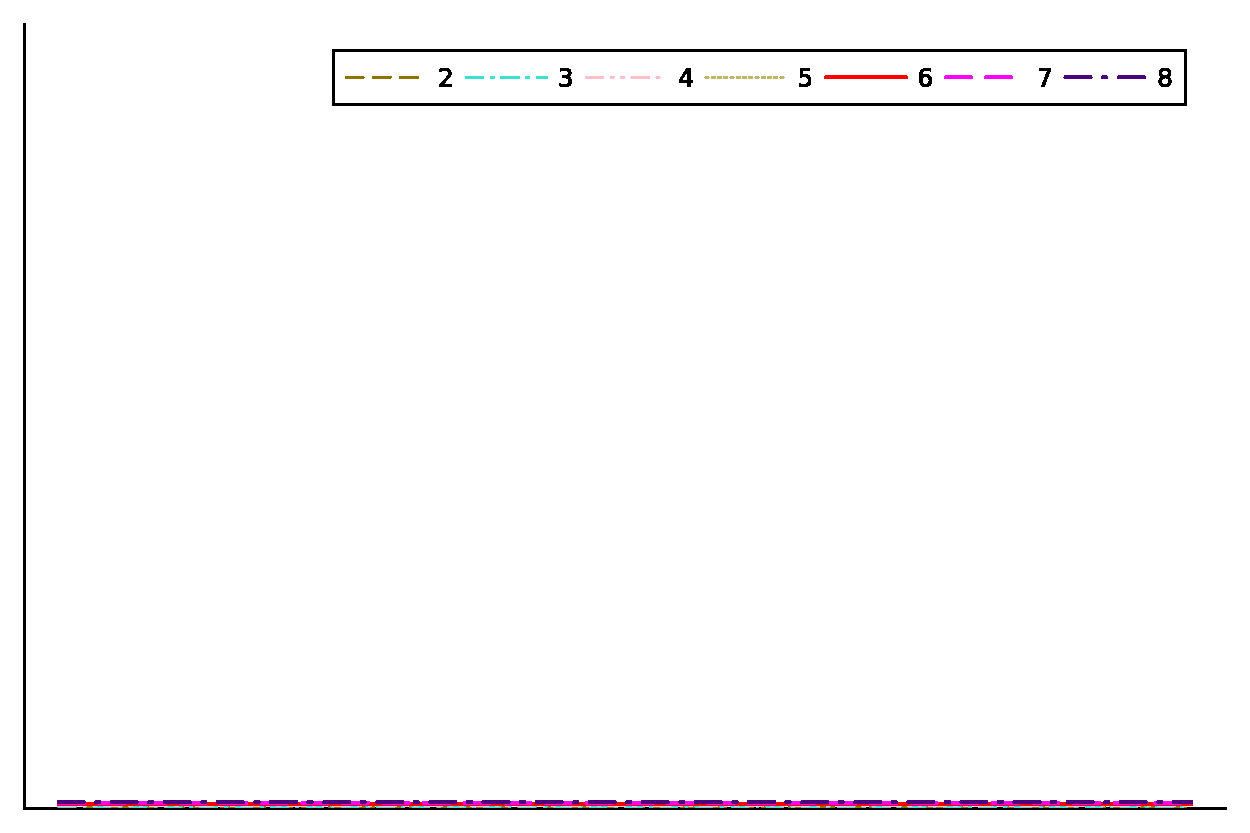
\includegraphics[width=0.5\textwidth,trim={160 340 30 22}, clip]{pdf/pdepics/legends/colors_a-d_new_horiz_2-8_no_order.pdf}\\	\begin{minipage}[t]{0.32\textwidth}
		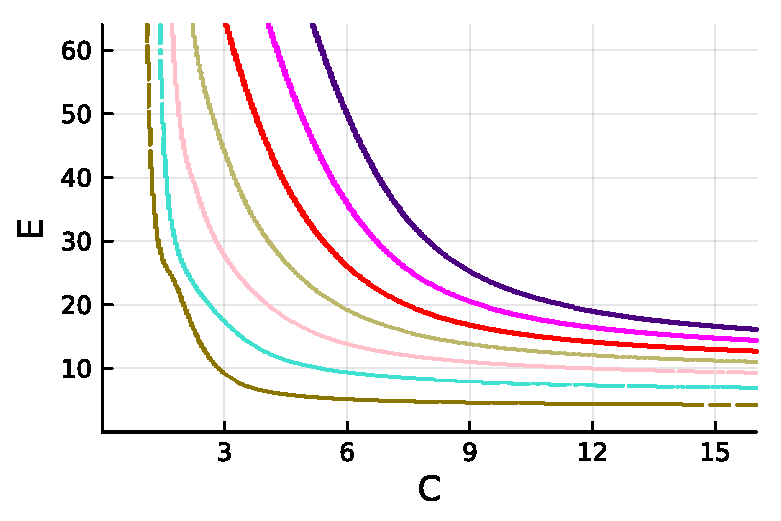
\includegraphics[width=\textwidth]{pdf/pdepics/diff/IMEXDeC_equispaced_TMM_ord_2-8.pdf}
		\centering
		IMEX DeC eq
	\end{minipage} 
	\begin{minipage}[t]{0.32\textwidth}
		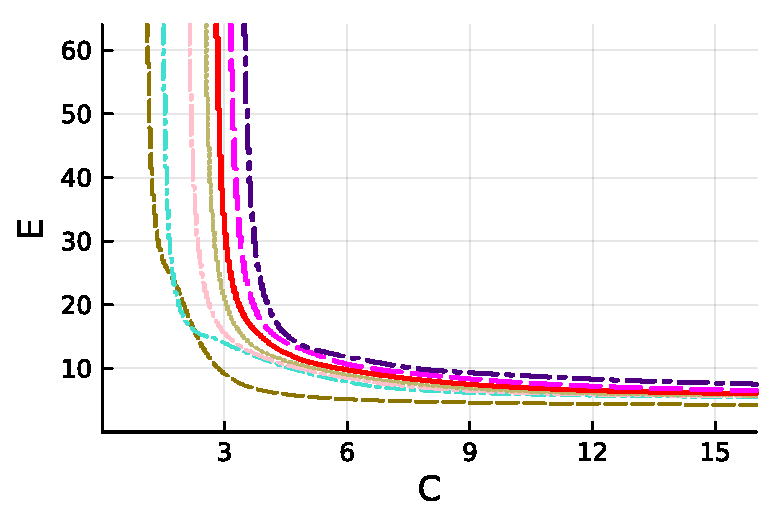
\includegraphics[width=\textwidth]{pdf/pdepics/diff/IMEXDeC_subtimesteps_equispaced_TMM_ord_2-8.pdf}
		\centering
		IMEX sDeC eq
	\end{minipage}
	\begin{minipage}[t]{0.32\textwidth}
		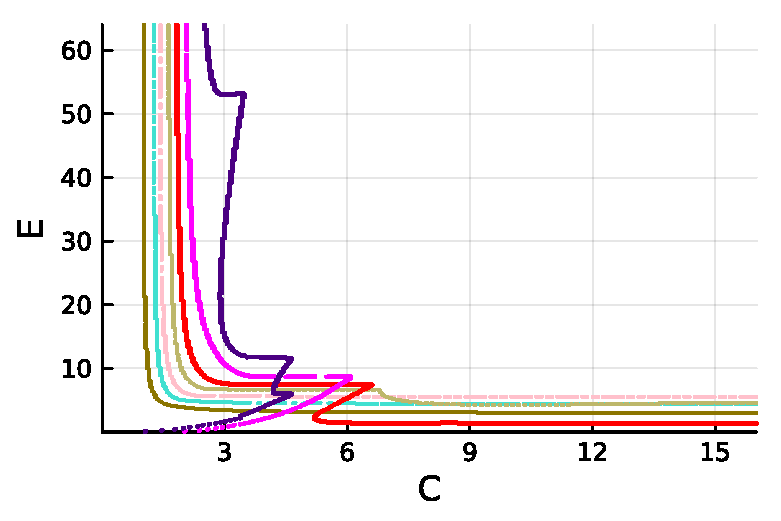
\includegraphics[width=\textwidth]{pdf/pdepics/diff/IMEXADER_equispaced_TMM_ord_2-8.pdf}
		\centering
		IMEX ADER eq
	\end{minipage} \\
	\begin{minipage}[t]{0.32\textwidth}
		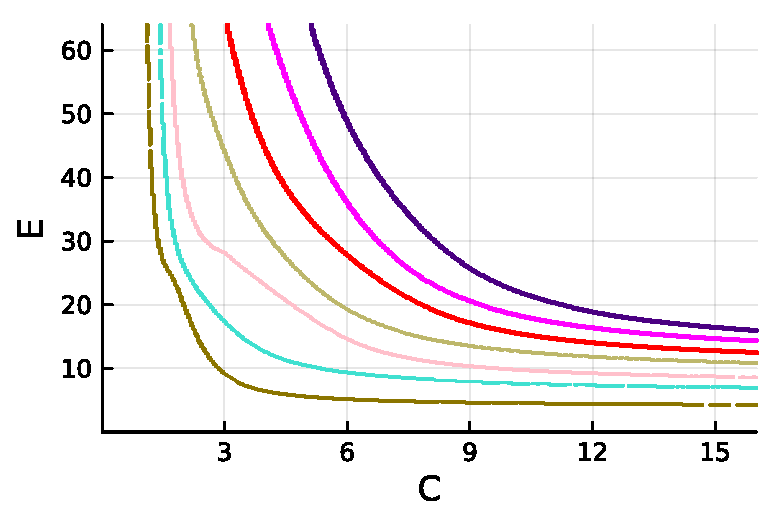
\includegraphics[width=\textwidth]{pdf/pdepics/diff/IMEXDeC_gaussLobatto_TMM_ord_2-8.pdf}
		\centering
		IMEX DeC GLB
	\end{minipage} 
	\begin{minipage}[t]{0.32\textwidth}
		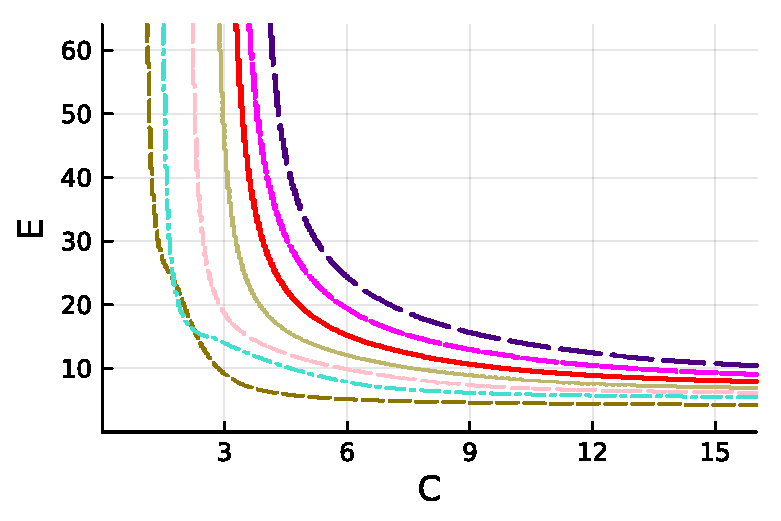
\includegraphics[width=\textwidth]{pdf/pdepics/diff/IMEXDeC_subtimesteps_gaussLobatto_TMM_ord_2-8.pdf}
		\centering
		IMEX sDeC GLB
	\end{minipage}
	\begin{minipage}[t]{0.32\textwidth}
		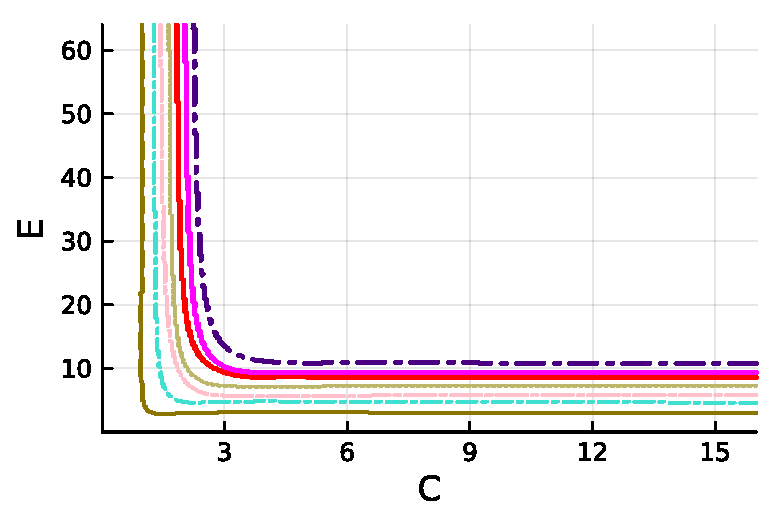
\includegraphics[width=\textwidth]{pdf/pdepics/diff/IMEXADER_gaussLobatto_TMM_ord_2-8.pdf}
		\centering
		IMEX ADER GLB
	\end{minipage} 
	\caption{Stability areas for $[\TMM,\NODES,k, A_1,D_2]$ for $\TMM$ as IMEX DeC (left), IMEX sDeC (center) and IMEX ADER (right) with eq (top) and GLB (bottom) nodes: $\TMM$ order $k$ from 2 to 8}
	\label{fig: grp_adv1_diff2}
\end{figure}

In the equispaced case we do not observe major differences for the DeC and sDeC methods, 
while, for the ADER cases, the usage of equispaced nodes results in an irregular reduction to $C_0=0$ for some orders (7 and 8), meaning that we can not assure stability as we did in the other cases for high order methods. 
This is probably impacted by the catastrophic cancellation which occurs in Newton-Cotes quadratures with more than 8 points that occur for orders larger than $6$, used in the considered IMEX ADER method. 
%The reason for this catastrophic cancellation effect lies in negative weights of the quadrature which firstly appear for 8 steps. 
%This hypothesis is also supported by the IMEX ADER in figure~\ref{fig: grp_adv1_diff2_GLB} with Gauss-Lobatto nodes, where this phenomenon does not appear.
For this reason, we will mainly analyze this method with Gauss-Lobatto nodes for the other cases.



In Figure~\ref{fig: exa_advterm}, we display the stability areas for the $[\DeC,\eq,8, A_k,D_2]$, $[\sDeC,\eq,8, A_k,D_8]$ and $[\ADER,\GLB,8, A_k,D_8]$ increasing the order for the finite difference scheme for the advection operator. 
For DeC (left), this does not lead to higher values for $E_0$ or $C_0$, but seemingly decreases for odd orders and increases for even orders, while starting with relatively big values for order 1 and relatively small values for order 2. 
It seems that they all guide towards a specific border line. It is also surprising that  we do not get a border $E_0>0$ for order 6 in the advection term for equispaced nodes, while we do for GLB ones (not displayed). 
These phenomena hold for all remaining combinations of time-marching methods, respective orders and nodes also, i.e. if we increase the order of the diffusion term, we can eliminate instabilities that occur due to the advection term, while the remaining variables just play a minor role. 
Exemplary, we display in Figure~\ref{fig: exa_advterm} on the right the $[\ADER,\GLB,8, A_k,D_2]$  to underline this statement. 
This is again not true for order 6 for which all time methods do not show a stability region of type $E\leq E_0$.
%The only exception we observed appears for the higher order ADER with equispaced nodes, as we already saw in figure \ref{fig: grp_adv1_diff2_eq} and is displayed for varying advection terms in figure \ref{fig: exa_advtermADER} on the right: Under these conditions, the instabilities remain.
\begin{figure}[!h]
	\centering
	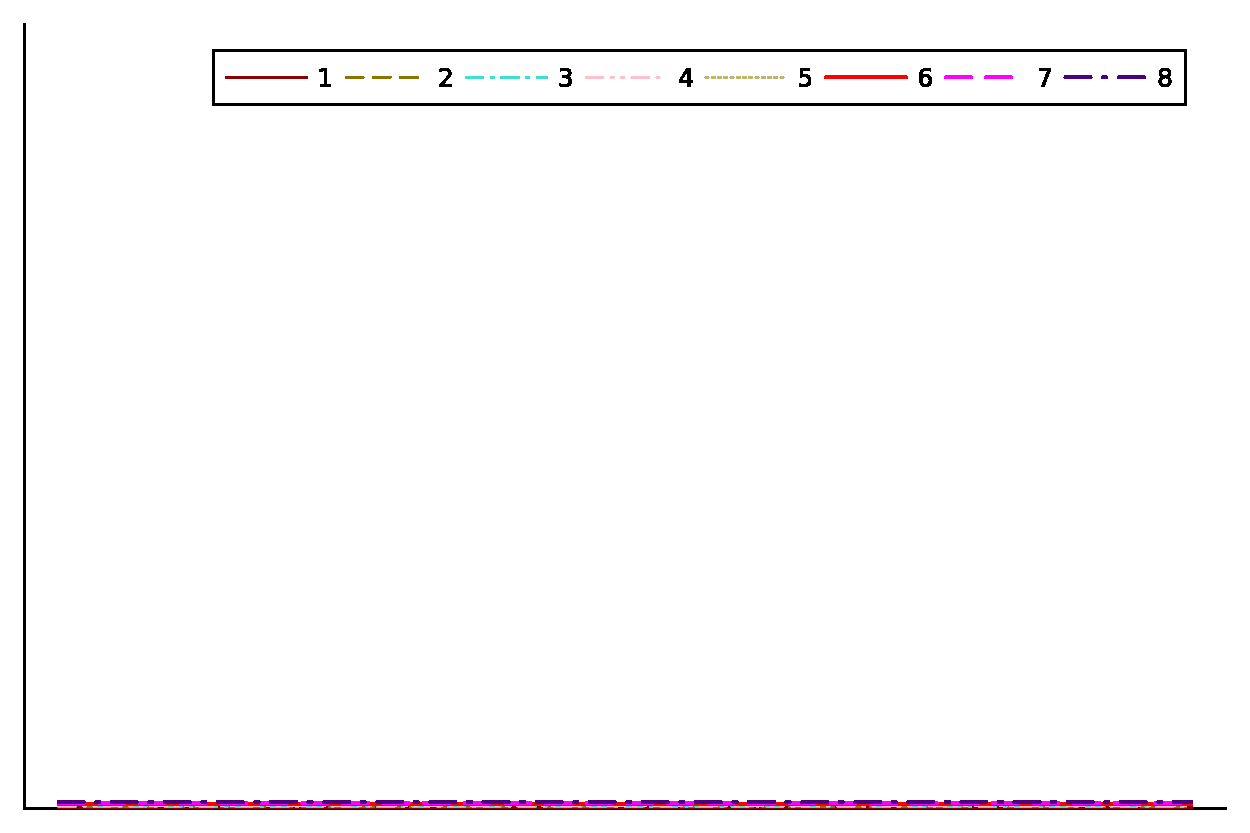
\includegraphics[width=0.6\textwidth,trim={100 340 30 22}, clip]{pdf/pdepics/legends/colors_a-d_new_horiz_1-8_no_order.pdf}\\
	\begin{minipage}[t]{0.32\textwidth}
		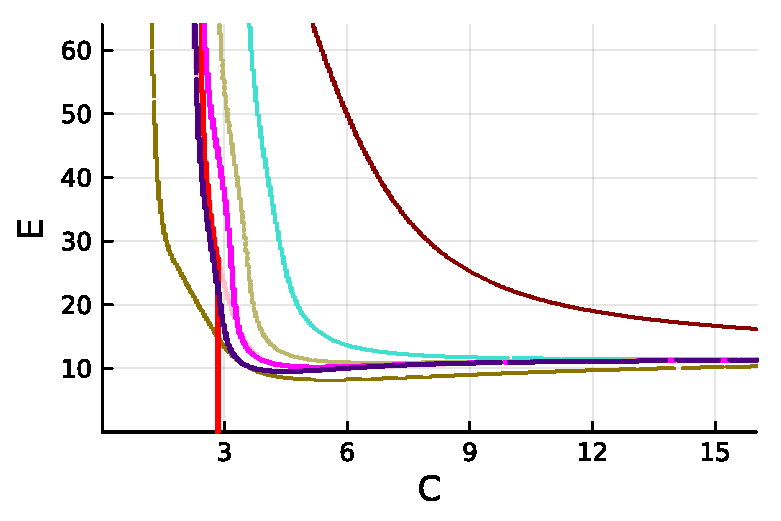
\includegraphics[width=\textwidth]{pdf/pdepics/diff/IMEXDeC_equispaced_adv_ord_1-8.pdf}
		\centering
		$[\DeC,\eq,8, A_k,D_2]$
	\end{minipage} 
	\begin{minipage}[t]{0.32\textwidth}
		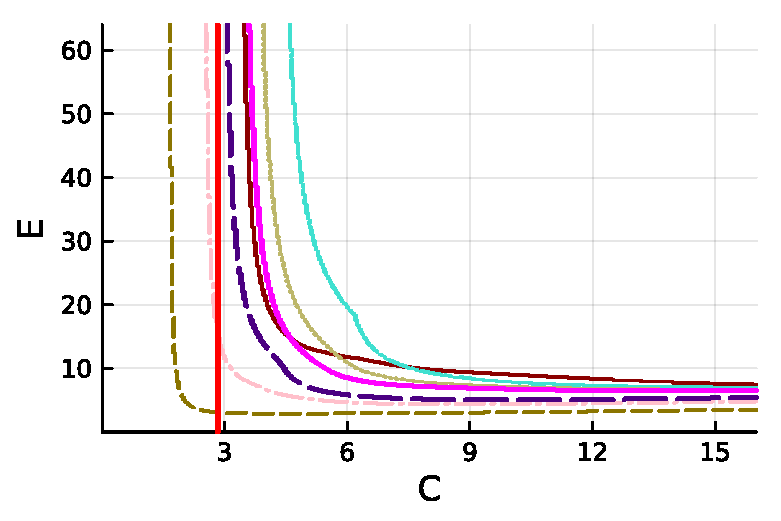
\includegraphics[width=\textwidth]{pdf/pdepics/diff/IMEXDeC_subtimesteps_equispaced_adv_ord_1-8.pdf}
		\centering
		$[\sDeC,\eq,8, A_k,D_2]$
	\end{minipage}
	\begin{minipage}[t]{0.32\textwidth}
		WAITING FOR PLOT!
		%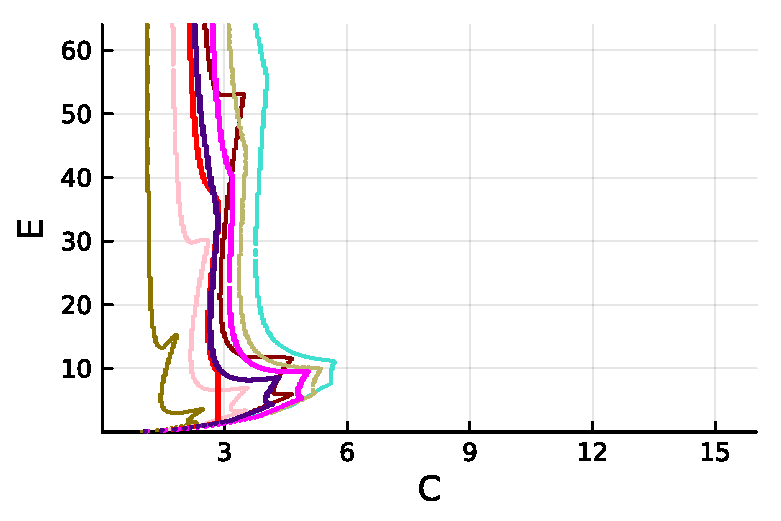
\includegraphics[width=\textwidth]{pdf/pdepics/diff/IMEXADER_equispaced_adv_ord_1-8.pdf}
		\centering
		$[\ADER,\eq,8, A_k,D_2]$
	\end{minipage}\\
	\begin{minipage}[t]{0.32\textwidth}
		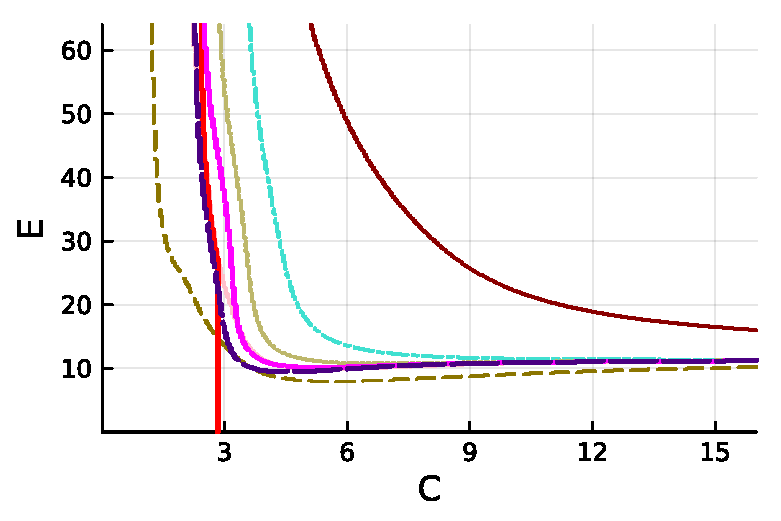
\includegraphics[width=\textwidth]{pdf/pdepics/diff/IMEXDeC_gaussLobatto_adv_ord_1-8.pdf}
		\centering
		$[\DeC,\GLB,8, A_k,D_2]$
	\end{minipage}
	\begin{minipage}[t]{0.32\textwidth}
		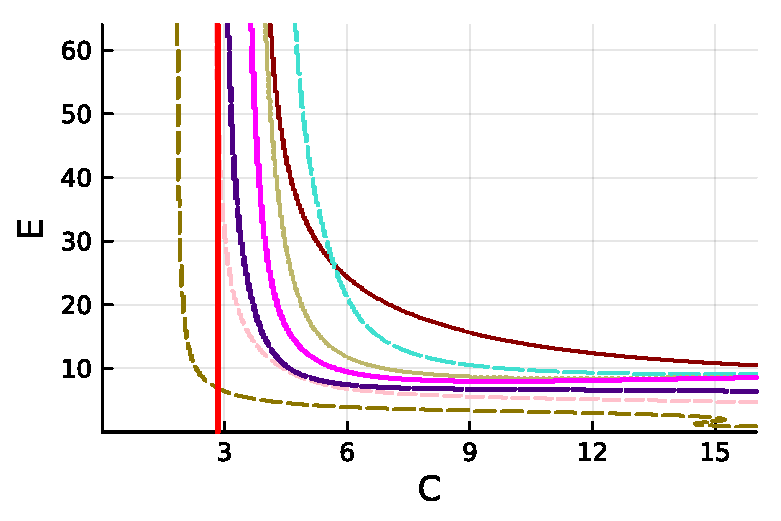
\includegraphics[width=\textwidth]{pdf/pdepics/diff/IMEXDeC_subtimesteps_gaussLobatto_adv_ord_1-8.pdf}
		\centering
		$[\sDeC,\GLB,8, A_k,D_2]$
	\end{minipage}
	\begin{minipage}[t]{0.32\textwidth}
		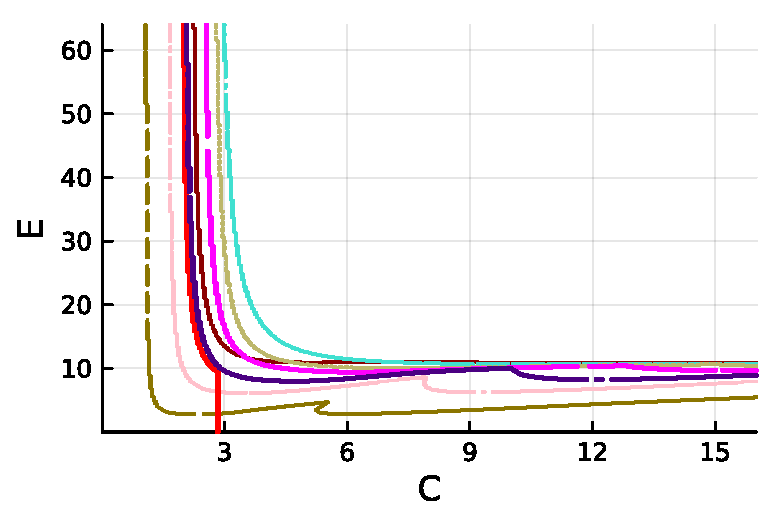
\includegraphics[width=\textwidth]{pdf/pdepics/diff/IMEXADER_gaussLobatto_adv_ord_1-8.pdf}
		\centering
		$[\ADER,\GLB,8, A_k,D_2]$
	\end{minipage}
	\caption{DeC Stability areas varying the order of the advection method}
	\label{fig: exa_advterm}
\end{figure}


In Figure~\ref{fig: exa_diffterm}, we show the stability regions increasing the order of the diffusion operator for $[\TMM,eq, 8, A_1,D_k]$, where $\TMM$ is every of the 3 considered methods and $k \in \{2,4,6,8\}$.  We observe that the stability areas of all methods vary slightly, but do not increase or decrease the stability region in a significant way.

\begin{figure}[!h]
	\centering
	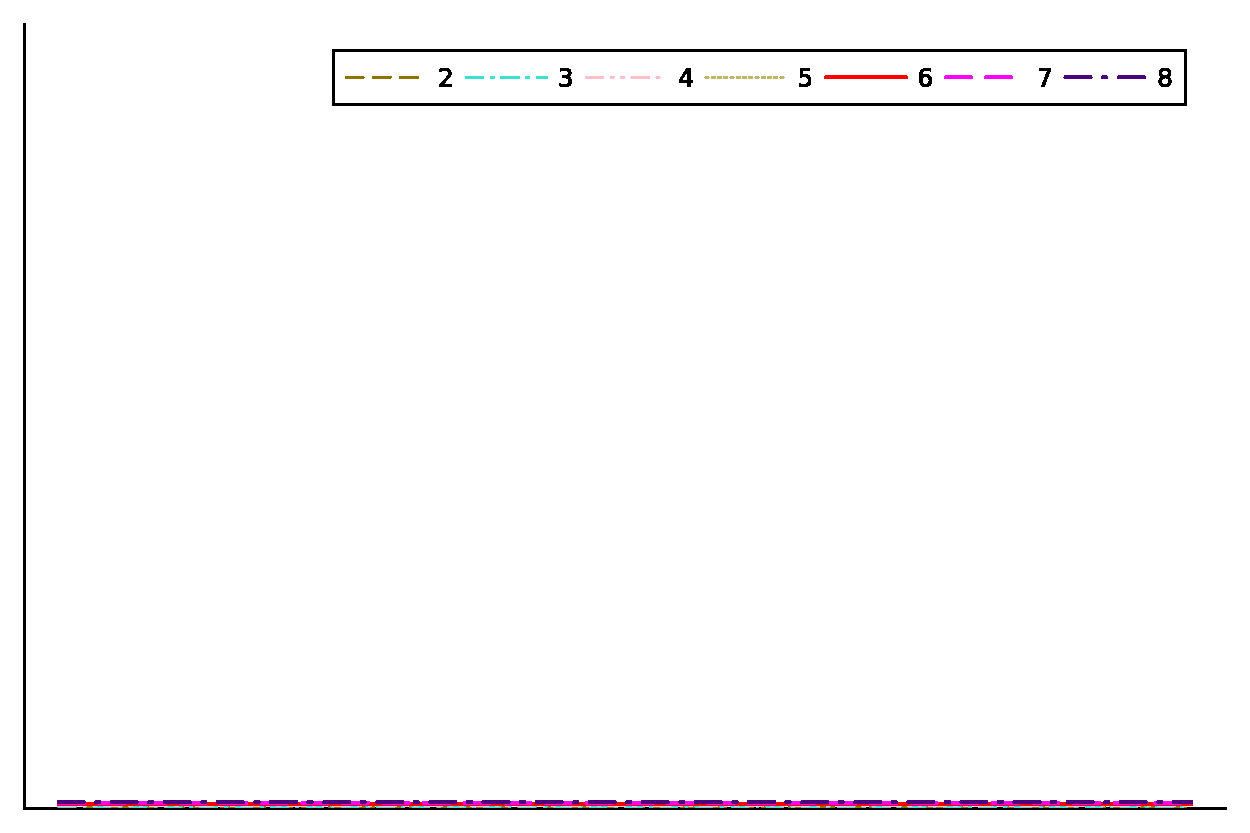
\includegraphics[width=0.6\textwidth,trim={160 340 30 22}, clip]{pdf/pdepics/legends/colors_a-d_new_horiz_2-8_no_order.pdf}\\
	\begin{minipage}[t]{0.32\textwidth}
		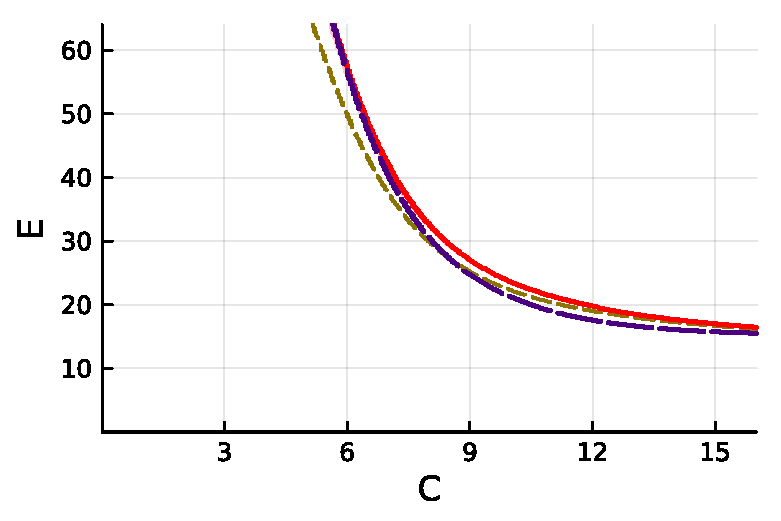
\includegraphics[width=\textwidth]{pdf/pdepics/diff/IMEXDeC_equispaced_diff_ord_2468.pdf}
		\centering
		$[\DeC,\eq, 8, A_1,D_k]$
	\end{minipage} 
	\begin{minipage}[t]{0.32\textwidth}
		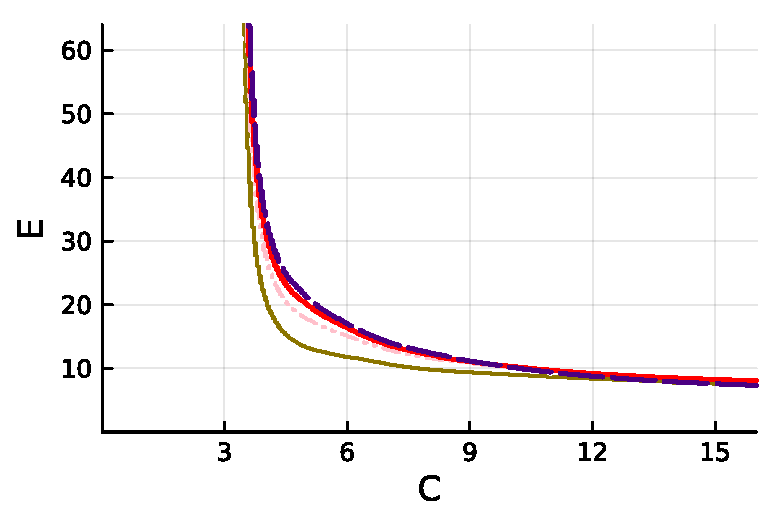
\includegraphics[width=\textwidth]{pdf/pdepics/diff/IMEXDeC_subtimesteps_equispaced_diff_ord_2468.pdf}
		\centering
		$[\sDeC,\eq, 8, A_1,D_k]$
	\end{minipage}
	\begin{minipage}[t]{0.32\textwidth}
		WAITING FOR PLOT
		%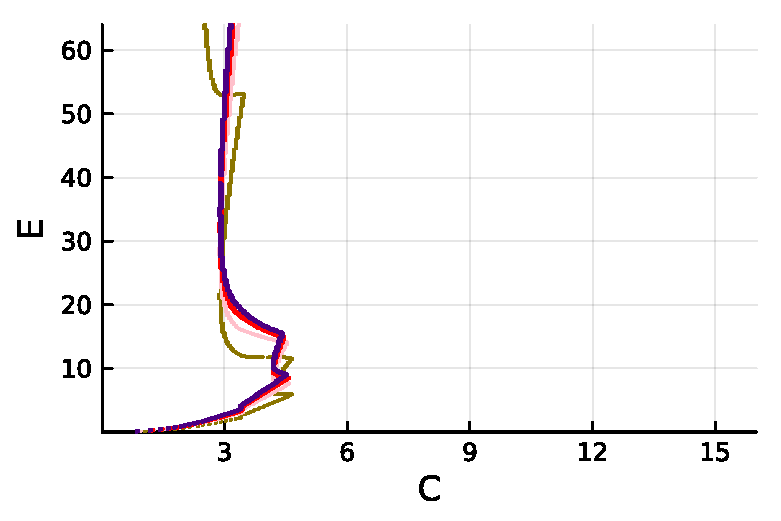
\includegraphics[width=\textwidth]{pdf/pdepics/diff/IMEXADER_equispaced_diff_ord_2468.pdf}
		\centering
		$[\ADER,\eq, 8, A_1,D_k]$
	\end{minipage}\\
	\begin{minipage}[t]{0.32\textwidth}
		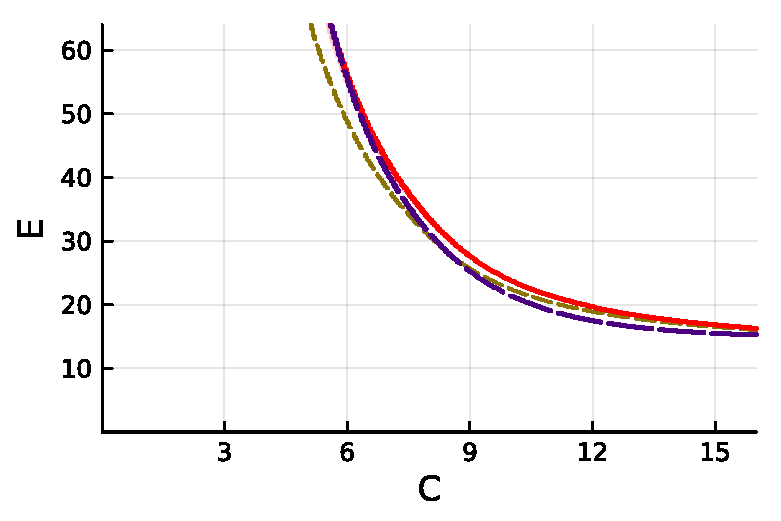
\includegraphics[width=\textwidth]{pdf/pdepics/diff/IMEXDeC_gaussLobatto_diff_ord_2468.pdf}
		\centering
		$[\DeC,\GLB, 8, A_1,D_k]$
	\end{minipage} 
	\begin{minipage}[t]{0.32\textwidth}
		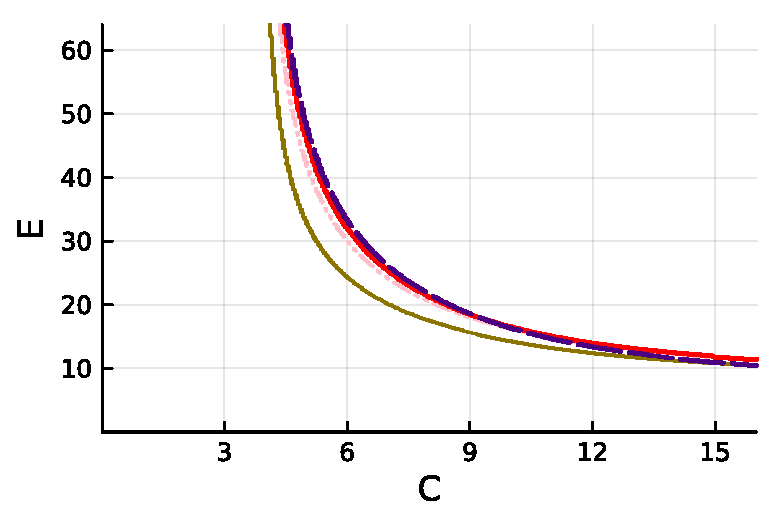
\includegraphics[width=\textwidth]{pdf/pdepics/diff/IMEXDeC_subtimesteps_gaussLobatto_diff_ord_2468.pdf}
		\centering
		$[\sDeC,\GLB, 8, A_1,D_k]$
	\end{minipage}
	\begin{minipage}[t]{0.32\textwidth}
		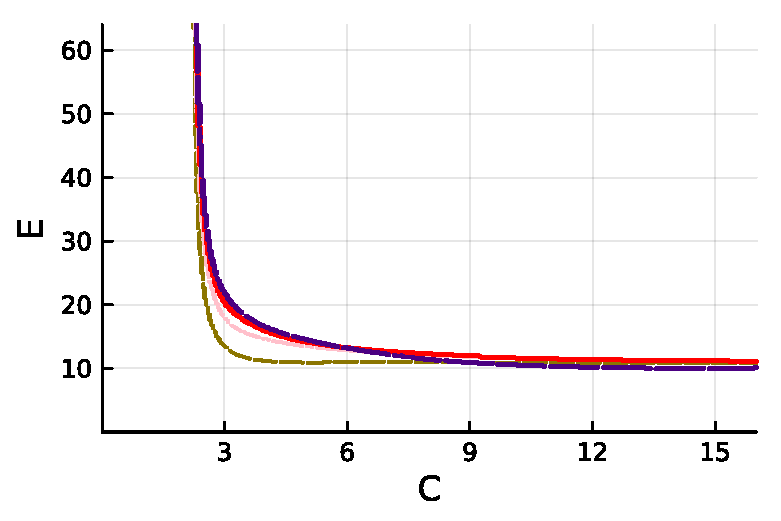
\includegraphics[width=\textwidth]{pdf/pdepics/diff/IMEXADER_gaussLobatto_diff_ord_2468.pdf}
		\centering
		$[\ADER,\GLB, 8, A_1,D_k]$
	\end{minipage}
	\caption{Stability areas varying the order of the diffusion method}
	\label{fig: exa_diffterm}
\end{figure}
\todo{The following paragraph would be rewritten shortly. There do not happen many new interesting things, just showing it works, giving a hint to the table and reminding that the instabilities for advection order 6 gets removes by matching the dispersion order}
In Figure~\ref{fig: exa_difftermsim}, we study the space--time discretizations matching the orders of the time scheme with the order of the spatial terms, i.e.  $[\TMM,\GLB, k, A_k,D_{2\lceil k/2 \rceil}]$, where $\TMM$ is one of the 3 considered methods and $k \in \{2, \hdots, 8\}$.
Here, we can observe for all cases that the higher order terms results in slightly larger stability areas and also in bigger $C_0$ and $E_0$, which leads us to the behavior we have already seen in Figure~\ref{fig: grp_adv1_diff2} varying only the order of the time scheme. 

\begin{figure}[!h]
	\centering
	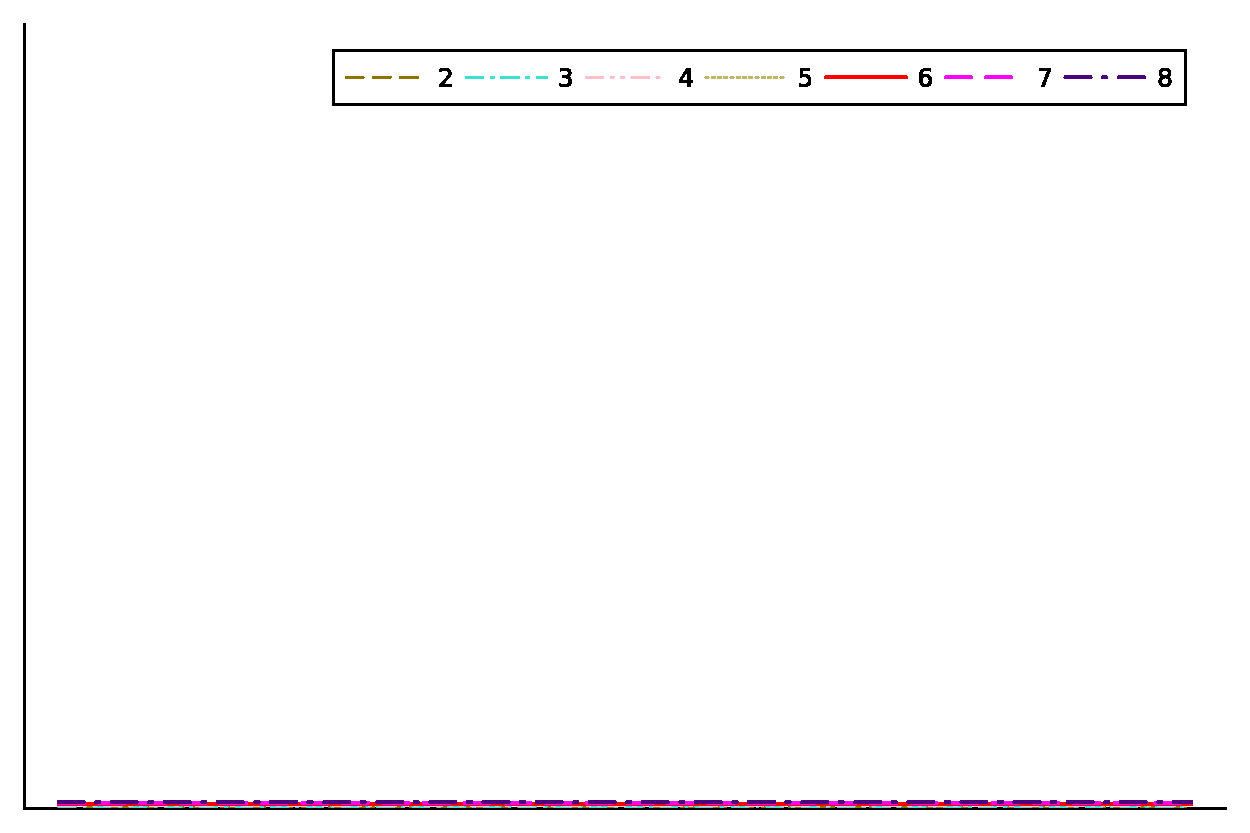
\includegraphics[width=0.6\textwidth,trim={160 340 30 22}, clip]{pdf/pdepics/legends/colors_a-d_new_horiz_2-8_no_order.pdf}\\
	\begin{minipage}[t]{0.32\textwidth}
		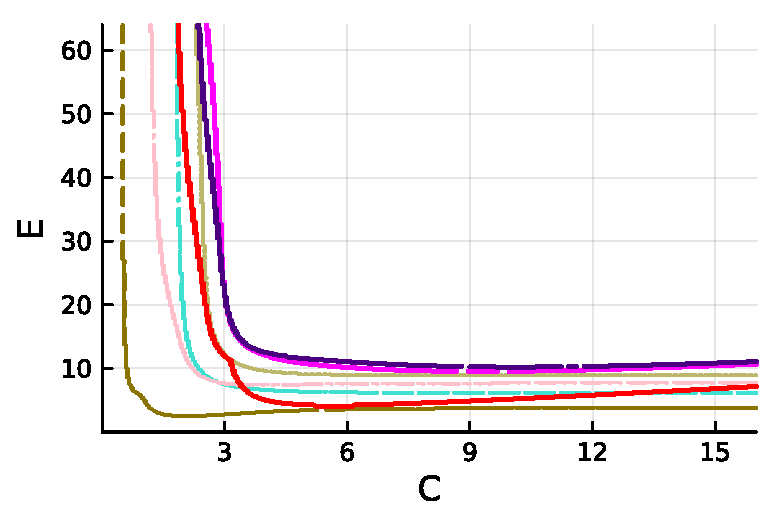
\includegraphics[width=\textwidth]{pdf/pdepics/diff/IMEXDeC_equispaced_all_2-8.pdf}
		\centering
		$[\DeC,\eq, k, A_k,D_{2\lceil k/2 \rceil}]$
	\end{minipage} 
	\begin{minipage}[t]{0.32\textwidth}
		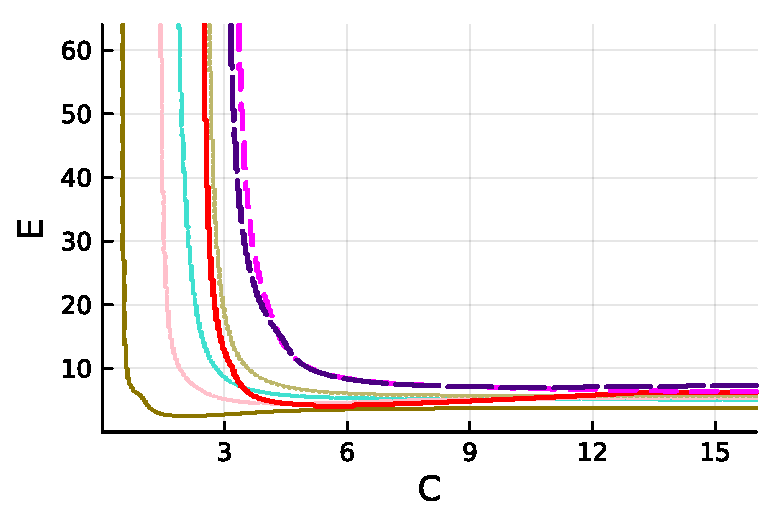
\includegraphics[width=\textwidth]{pdf/pdepics/diff/IMEXDeC_subtimesteps_equispaced_all_2-8.pdf}
		\centering
		$[\sDeC,\eq, k, A_k,D_{2\lceil k/2 \rceil}]$
	\end{minipage}
	\begin{minipage}[t]{0.32\textwidth}
		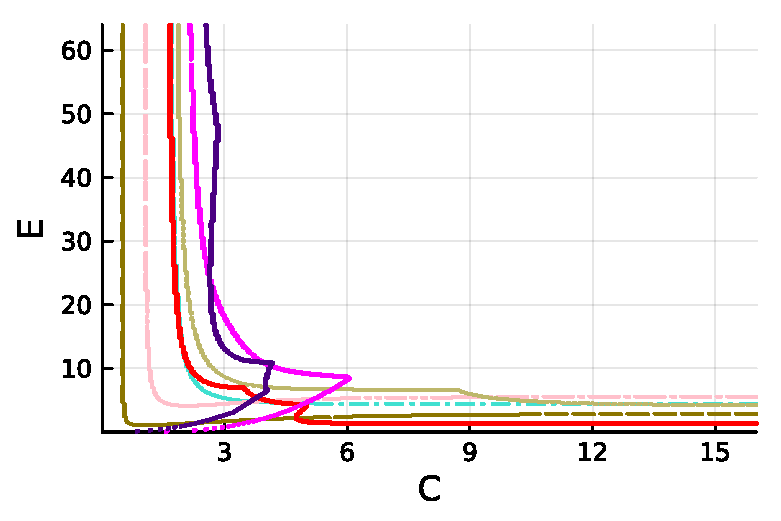
\includegraphics[width=\textwidth]{pdf/pdepics/diff/IMEXADER_equispaced_all_2-8.pdf}
		\centering
		$[\ADER,\eq, k, A_k,D_{2\lceil k/2 \rceil}]$
	\end{minipage}\\
	\begin{minipage}[t]{0.32\textwidth}
		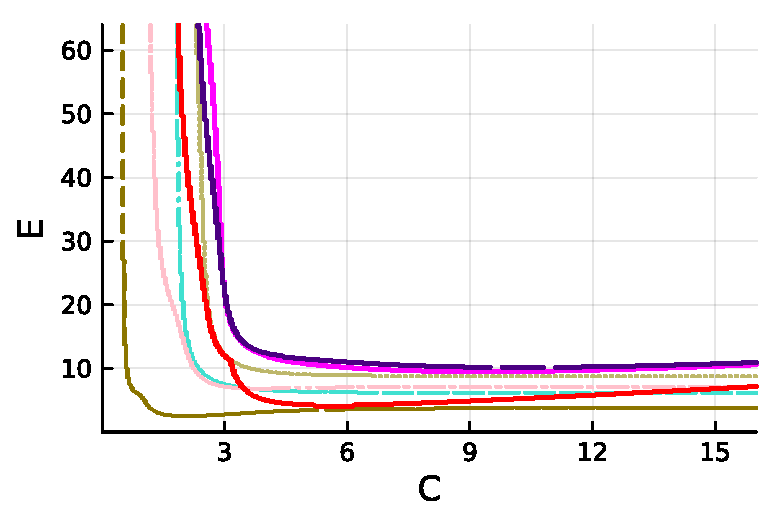
\includegraphics[width=\textwidth]{pdf/pdepics/diff/IMEXDeC_gaussLobatto_all_2-8.pdf}
		\centering
		$[\DeC,\GLB, k, A_k,D_{2\lceil k/2 \rceil}]$
	\end{minipage} 
	\begin{minipage}[t]{0.32\textwidth}
		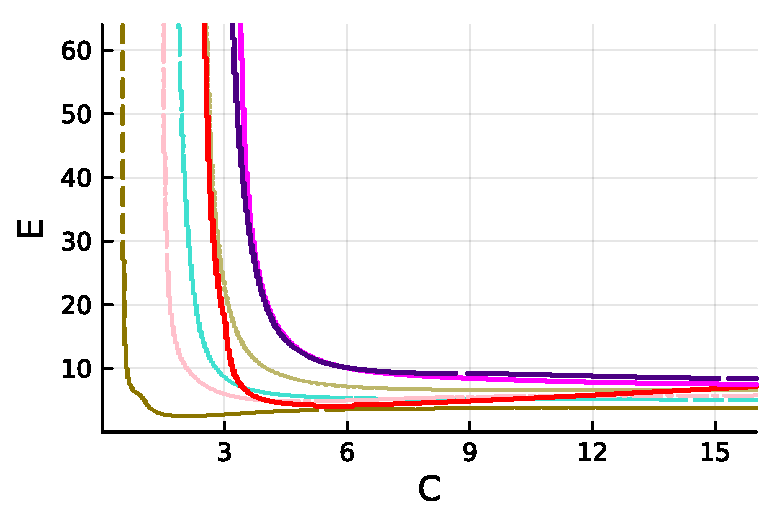
\includegraphics[width=\textwidth]{pdf/pdepics/diff/IMEXDeC_subtimesteps_gaussLobatto_all_2-8.pdf}
		\centering
		$[\sDeC,\GLB, k, A_k,D_{2\lceil k/2 \rceil}]$
	\end{minipage}
	\begin{minipage}[t]{0.32\textwidth}
		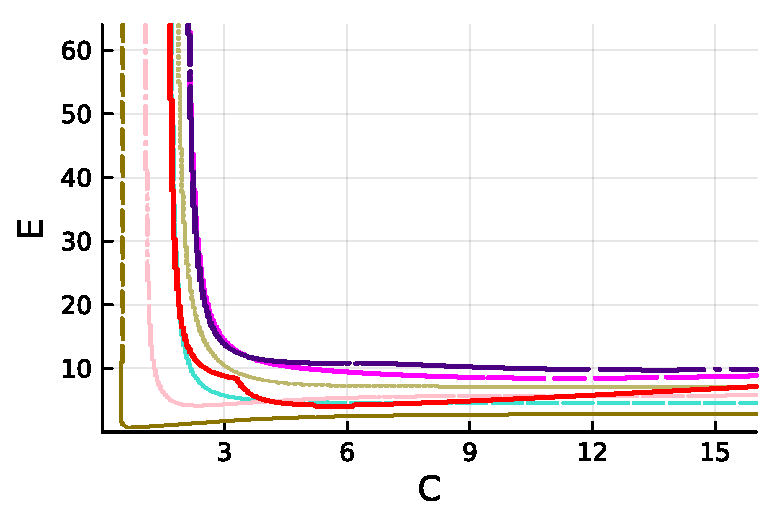
\includegraphics[width=\textwidth]{pdf/pdepics/diff/IMEXADER_gaussLobatto_all_2-8.pdf}
		\centering
		$[\ADER,\GLB, k, A_k,D_{2\lceil k/2 \rceil}]$
	\end{minipage}	
	\caption{Stability areas varying the order of all partial methods.}
	\label{fig: exa_difftermsim}
\end{figure}

We can conclude that increasing the order of the time-marching method results in higher values for both $C_0$ and $E_0$. However, the here considered higher order finite differences for the spatial discretizations do not grant significant improvements. In the recent analysis, the border $E_0$ vanishes for the special setting IMEX ADER of order $>7$  with equispaced nodes, independently of the spatial discretization we used. We also get this phenomenon by setting the advection stencil to order 6, but this problem can be overcome by the usage of high order diffusion stencils.\\
Remark also, that there are plenty more options to test, which we leave out because of space restrictions. Nevertheless, we presented all remarkable combinations of methods we tested and a summary of their results.

\begin{table}
	\centering
	\caption{Approximated border values $C_0$ (up to 2 decimals) and $E_0$ (up to 1 decimal) for Gauss--Lobatto methods with operators with optimal order $k$}\label{tab:CE_values}
	\begin{tabular}{|c||c|c||c|c||c|c|}\hline
				$k$&
		\multicolumn{2}{|c||}{$[\DeC,\GLB,k,A_k,D_{2\lceil k/2 \rceil}]$}&
		\multicolumn{2}{|c||}{$[\sDeC,\GLB,k,A_k,D_{2\lceil k/2 \rceil}]$}&
		\multicolumn{2}{|c|}{$[\ADER,\GLB,k,A_k,D_{2\lceil k/2 \rceil}]$}\\\hline
		&$\qquad C_0\qquad$&$E_0$&$\qquad C_0\qquad$&$E_0$&$\qquad C_0\qquad$&$E_0$\\\hline
		2& 0.50 &2.5&0.50&2.5&0.50&0.7\\
		3& 1.63 &6.1&1.69&5.1&1.63&4.5\\
		4& 1.04&6.9&1.43&4.9&1.04&4.2\\
		5& 1.74&8.8&2.31&6.6&1.74&7.2\\
		6& 1.60&4.1&2.33&4.2&1.60&4.1\\
		7& 1.94&9.5&3.12&7.5&1.94&8.5\\
		8&2.00&10.2&2.85&5.9&2.00&9.8\\ \hline
	\end{tabular}
\end{table}

In Table~\ref{tab:CE_values}, we study the operators with order $k$ matching for the time and spatial discretization for time schemes defined by GLB nodes. We display in that table the maximal values $C_0$ and $E_0$. 
We clearly see that they increase as the order increases. 
The only value that is not uniform among the methods is $E_0$ for ADER GLB of order 2, for which we have a restrictive bound.